%%%%%%%%%%%%%%%%%%%%%%%%%%%%%%%%%%%%%%%%%%%%%%%%%%%%%%%%%%%%%%%%%%%%%%%%%%%%
%% Author template for INFORMS Journal on Optimization (ijoo) 
%%   [interim solution; new styles under construction]
%% Mirko Janc, Ph.D., INFORMS, mirko.janc@informs.org
%% ver. 0.93, November 2017
%%%%%%%%%%%%%%%%%%%%%%%%%%%%%%%%%%%%%%%%%%%%%%%%%%%%%%%%%%%%%%%%%%%%%%%%%%%%
\documentclass[ijoo,nonblindrev]{informs-ijoo}

\OneAndAHalfSpacedXI
%%\OneAndAHalfSpacedXII % Current default line spacing
%%\DoubleSpacedXII
%%\DoubleSpacedXI

% Private macros here (check that there is no clash with the style)

% Natbib setup for author-year style
\usepackage{natbib}
 \bibpunct[, ]{(}{)}{,}{a}{}{,}%
 \def\bibfont{\small}%
 \def\bibsep{\smallskipamount}%
 \def\bibhang{24pt}%
 \def\newblock{\ }%
 \def\BIBand{and}%
\usepackage{comment}
\usepackage{xcolor}
\usepackage[linesnumbered,ruled,vlined]{algorithm2e}
\usepackage{amsmath}
\usepackage{soul}
%% Setup of theorem styles. Outcomment only one.
%% Preferred default is the first option.
\TheoremsNumberedThrough     % Preferred (Theorem 1, Lemma 1, Theorem 2)
%\TheoremsNumberedByChapter  % (Theorem 1.1, Lema 1.1, Theorem 1.2)
\ECRepeatTheorems

%% Setup of the equation numbering system. Outcomment only one.
%% Preferred default is the first option.
\EquationsNumberedThrough    % Default: (1), (2), ...
%\EquationsNumberedBySection % (1.1), (1.2), ...

% For new submissions, leave this number blank.
% For revisions, input the manuscript number assigned by the on-line
% system along with a suffix ".Rx" where x is the revision number.
\MANUSCRIPTNO{MS-0001-1922.65}

%%%%%%%%%%%%%%%%
\begin{document}
%%%%%%%%%%%%%%%%

% Outcomment only when entries are known. Otherwise leave as is and
%   default values will be used.
%\setcounter{page}{1}
%\VOLUME{00}%
%\NO{0}%
%\MONTH{Xxxxx}% (month or a similar seasonal id)
%\YEAR{0000}% e.g., 2005
%\FIRSTPAGE{000}%
%\LASTPAGE{000}%
%\SHORTYEAR{00}% shortened year (two-digit)
%\ISSUE{0000} %
%\LONGFIRSTPAGE{0001} %
%\DOI{10.1287/xxxx.0000.0000}%

% Author's names for the running heads
% Sample depending on the number of authors;
% \RUNAUTHOR{Jones}
\RUNAUTHOR{de Lemos and Woodward}
% \RUNAUTHOR{Jones, Miller, and Wilson}
% \RUNAUTHOR{Jones et al.} % for four or more authors
% Enter authors following the given pattern:
%\RUNAUTHOR{}

% Title or shortened title suitable for running heads. Sample:
% \RUNTITLE{Bundling Information Goods of Decreasing Value}
% Enter the (shortened) title:
\RUNTITLE{A Constructive Heuristic for the Aircraft Recovery Problem}

% Full title. Sample:
% \TITLE{Bundling Information Goods of Decreasing Value}
% Enter the full title:
\TITLE{A Constructive Heuristic for the Aircraft Recovery Problem}

% Block of authors and their affiliations starts here:
% NOTE: Authors with same affiliation, if the order of authors allows,
%   should be entered in ONE field, separated by a comma.
%   \EMAIL field can be repeated if more than one author
\ARTICLEAUTHORS{%
\AUTHOR{Francisco de Lemos}
\AFF{School of Electronic Engineering and Computer Science, Queen Mary University of London, 10 Godward Square, Mile End Rd, Mile End, London E1 4FZ, \EMAIL{f.j.r.lemos@qmul.ac.uk}} %, \URL{}}
\AUTHOR{John Woodward}
\AFF{School of Electronic Engineering and Computer Science, Queen Mary University of London, 10 Godward Square, Mile End Rd, Mile End, London E1 4FZ, \EMAIL{j.woodward@qmul.ac.uk}}
% Enter all authors
} % end of the block

\ABSTRACT{%% Enter your abstract
An aircraft rotation consists of assigning flights to aircraft in such a way that operational constraints, such as maintenance, flight continuity, turn-round time, and airport capacity, are satisfied. However, aircraft rotations are often subject to disruption such as flight delay or cancellations, originated by inclement weather,
industrial action, or malfunctions. The Aircraft Recovery Problem (ARP) consists of altering the planned flight schedule to compensate the disruptions that resulted in the temporary or permanent unavailability of aircraft. In this work, we propose a recovery procedure for each disrupted rotation that starts by finding the first infeasible flight. We split the rotation in two sub-rotations, the first which is feasible, and the second where one or more constraints are not satisfied. For the second sub-rotation, the algorithm finds if the flights can be canceled and the time slots available to operate the flight. These values consist of the flight domains and by calculating the cartesian product of these domains we derive the search space for the second sub-rotation.
Depending on the size of the search space, the algorithm uses the upper heuristic to find solutions above a certain size of the search space or the lower heuristic to find solutions below a certain size of the search space.
For each iteration over the aircraft rotation, the algorithm will perform a pincer movement by simultaneously decreasing the upper bound and increasing the lower bound, thus closing in on a solution that complies with all the constraints. During the recovery procedure, the algorithm introduces new flights to replace those that were initially cancelled and taxi flights to reconnect the two sub-rotations. We present results for the solution cost and computing time for the Constructive Heuristic for the Aircraft Recovery Problem (CHARP) for various time windows and the introduction of new flights and taxi flights.
}

% Sample
%\KEYWORDS{deterministic inventory theory; infinite linear programming duality;
%  existence of optimal policies; semi-Markov decision process; cyclic schedule}

% Fill in data. If unknown, outcomment the field
\KEYWORDS{Constraint satisfaction, aircraft, disruption, recovery} 
%\HISTORY{This paper was
%first submitted on December 12, 2020 and has been with the authors for
%83 years for 65 revisions.}

\maketitle
%%%%%%%%%%%%%%%%%%%%%%%%%%%%%%%%%%%%%%%%%%%%%%%%%%%%%%%%%%%%%%%%%%%%%%

% Samples of sectioning (and labeling) in MNSC
% NOTE: (1) \section and \subsection do NOT end with a period
%       (2) \subsubsection and lower need end punctuation
%       (3) capitalization is as shown (title style).
%
%\section{Introduction.}\label{intro} %%1.
%\subsection{Duality and the Classical EOQ Problem.}\label{class-EOQ} %% 1.1.
%\subsection{Outline.}\label{outline1} %% 1.2.
%\subsubsection{Cyclic Schedules for the General Deterministic SMDP.}
%  \label{cyclic-schedules} %% 1.2.1
%\section{Problem Description.}\label{problemdescription} %% 2.

% Text of your paper here

\section{Introduction}

The financial objective of airline companies is maximizing their profits while operating flights according to a schedule. Therefore, airlines create tight schedules to increase their profitability. These tight schedules, have a minimum slack between flights legs, because they rely on the assumption that the flight legs will be operated as planned. A rotation consists in assigning an aircraft to a flight schedule while complying with operational constraints such as, aircraft maintenance, flight continuity, turn-round time and airport capacity for departure and arrival. Flight operations are on many occasions subject to irregularities that can complicate its execution. 

A considerable number of factors, such as mechanical failures, crew delays, problems with ground operations, industrial action, inclement weather, congestion at airports can cause disruptions such as flight delays or cancellations. As a result, the initial rotation becomes inefficient in the sense that flights must be delayed or cancelled. Since airline companies are liable to pay compensation for the resulting passenger inconvenience in these situations, leading to a negative financial impact on an airline’s profits, it thus becomes of the most importance to resume normal operations as quickly as possible. 



In case of disruptions, it is necessary to recover the rotation during the period of time designated by the recovery time window (RTW). During the RTW a feasible rotation must be found that mitigates the impact of disruptions. This is process called disruption recovery.

Disruption recovery is a real-time practice that requires finding a fast solution when irregularities occur. Often, disruptions take place during operations ($i.$ $e.$, only in few cases, it is possible to know a disruption in-advance), and a provisional plan must be provided quickly. Thus, it is necessary to construct efficient algorithms to have feasible solutions in minutes, moreover because when disruptions occur, they can affect more than just the directly disrupted flight and can send a shockwave of disruptions through the network.

It is during RTW’s duration that actions should be implemented to re-plan usage of resources all over the entire network of flights. The objective is to find a solution with minimal flight cancellation and delay, while meeting the constraints associated with flight time, aircraft or airport capacity and passenger itineraries. In this paper we will focus solely in recovering the aircraft rotation, also known as the aircraft recovery problem (ARP). To achieve this objective, we will use the data sets for the ROADEF 2009 Challenge. 
\begin{comment}
Every two years the \textit{French society of Operational Research and Decision Making} releases the ROADEF Challenge, which consists on a competition to solve a complex optimization problem that occurs in industry. In the ROADEF 2009 Challenge there is a step-wise simplification of a model, for disruption management in commercial aviation that aims at finding recovery planning of flights, aircraft assignments and passengers (including flight leg cancellation) on a given maximal horizon, so that a sum of penalties corresponding to various costs or discomforts is minimized. The present work is based on ROADEF 2009 Challengee and intends to develop a series of methodologies that will result in the generation of recovery processes for the disruptions induced by flight delays or cancellations, aircraft availability shortage or airport capacity decrease.\\

After retrieving the results for the ARRP using our algorithm, we will validate it using a flight schedule based on citep francis2020
\end{comment}


The remainder of the paper is organized as follows: an overview of the relevant literature is provided in Section \ref{sec:litRev}; the model for the aircraft  recovery problem is provided in Section \ref{sec:modelARP}; the  CHARP will be described in detail in Section \ref{sec:algorithms}; the computational results will be presented in Section \ref{sec:compResults}; the conclusions will be drawn in Section \ref{sec:conclusions}.


\section{Literature Review}\label{sec:litRev}


During the years several methodologies have been developed several approaches to tackle unpredicted irregularities that often cause disruptions in elaborately generated flight schedules.
 
%%%%%%%%%%%%%%%%%%%%%%%%%%%%%%%
\begin{comment}
 We first present in Section} \ref{sec:aircRecovery} \hl{an extensive literature review regarding the different methods used in the past thirty five years to perform aircraft recovery. In Section} \ref{sec:integratedRecovery} \hl{ we focus in reviewing the the methods that integrate the the ARP with passenger recovery problem (PRP), in particular, since we are using the ROADEF 2009 Challenge data sets, we will provide the literature review of the methods used in this competition.}
%%%%%%%%%%%%%%%%%%%%%%%%%%%%%%%%
%%%%%%%section Aircraft Recovery
%%%%%%%%%%%%%%%%%%%%%%%%%%%%%%%%
\subsection{Aircraft Recovery}\label{sec:aircRecovery}
\end{comment}
%%%%%%%%%%%%%%%%%%%%%%%%%%%%%%%
As reviewed by \citep{TEODOROVIC1984}, the authors developed a network model that minimizes the total passenger delay on an airline network and solved the problem of finding new routing and scheduling plan to optimality using a branch and bound heuristic. The authors model passenger delays explicitly but they assume that all passenger itineraries contain only a single flight leg. Given the considerable number of routings for even modest sized problems, it is doubtful that their approach could be materialized for practical problems. On the other hand, since companies manage their operations using hub and spoke flights, this study would also have limited scope of application.

\citep{Jarrah1993} present an overview of a decision support system for the aircraft recovery problem with the attempt of conceptualizing the problem. The authors used a minimum cost network models, one delay model and one cancellation model and implemented an algorithm that solves the shortest path problem repeatedly to determine the necessary flows. One of the major drawbacks of this work consists of not having solutions that combine both flight delay and cancellation.
\citep{Yan1997} developed a framework to help carriers handle schedule perturbation, due to temporary closure of airports, and resume their normal services as possible. This framework is based in a time-space network flow model, where the arcs in the network represent airborne flights, grounded flights, and overnight connections. The research was conducted over a set of scenarios, mathematically formulated either as pure network flow problems or network flow problems with side constraints, the former solved using simplex method and the latter using a Lagrangian relaxation-base algorithm, respectively. These models minimize the schedule-perturbed time after incidents so that carriers can resume their normal services as soon as possible. The salient features of the models consist in combining systematically flight cancellations, flight delays, the modification of multi-stop flights, the ferrying of idle aircraft and the swapping of aircraft. This procedure aims at adjusting effectively a schedule following incidents, so that a carrier can maintain its profitability.  The authors confine the scope of this research to the operations of a single fleet as well as simplifying multi-leg flights by considering that the time block is from the beginning of the first leg to the end of the last leg.\\
\citep{Cao1997-I} and \citep{Cao1997-II} extended the work developed by \cite{Jarrah1993} evaluating solutions with flight cancellations and delays. The authors used a linear programming approximation algorithm based on   a quadratic programming model that included both flight delays and cancellations. One of the major limitations of this work relates to the approach being limited to aircraft assigned to routes containing at most two flight legs.\\
The research led by \citep{Arguello1997} used a greedy randomized adaptive search procedure (GRASP) meta-heuristic to minimize flight cancellation and delay costs associated with a recovery aircraft routing, as a response to groundings and delays. The GRASP described in the study is adapted for use as a randomized neighbourhood search technique. In the procedure, the neighbours of an addressed solution are evaluated, and the most desirable are placed on a restructured candidate list. Neighbour generation operations are performed on pairs of aircraft routes. The authors introduced a series of constraints to enforce the model to share operational practices namely that, every flight in each aircraft route must depart from the airport where its previous flight arrived (balance constraint), a minimum turn-round time must be enforced between each flight arrival and subsequent departure, the recovery period extends to the end of the current day, aircraft must be positioned at the end of the recovery period in a specific airport so that the flight schedule can be resumed next day, airport departures are restricted in the curfew period and aircraft with planned maintenance will not have their original route altered. The approach was tested on data supplied by $Continental$ $Airlines$ and the results proved that the GRASP could produce in  most cases optimal or near-optimal solutions.\\
\citep{THENGVALL2000} solves the aircraft recovery problem for a single fleet over the entire flight schedule with an objective function that accounts for flight revenues, delays, cancellations, and an incentive to minimize deviations from the original schedule. The objective function consists in minimizing total operating costs, but crew and passenger disruptions are not considered. The problem is modelled using a time-space network and solved as an integer linear program using an optimization software.  To  represent the delays for a particular flight leg, a series  of delay arcs are introduced to consider the available options for later flights.  To  ensure   that only a single flight is chosen, a side constraint must be added requiring that the sum   for all arcs representing the same flight is less or equal to one. The model was able to accommodate recovery periods of arbitrary length that begin and end at arbitrary periods of the day. In addition, a rounding heuristic is introduced to obtain feasible integer solutions from the linear programming relaxation of the mixed-integer programming formulation. As mentioned by the authors one weakness of the model is that it does not track individual passengers and thus does not consider passenger connections. As for aircraft maintenance requisites the authors chose to remove aircraft due for maintenance from delays or cancellations to assure they reach their proper destination. This work was extended in \citep{Thengvall2001} by solving the multi-fleet aircraft schedule recovery, using multi-commodity network-type models during a hub closure.\\
\citep{Love2001} defined the dedicated aircraft recovery problem (DARP) as \textit{given an original flight schedule and one or more disruptions, the DARP consists of changing  the flight assignments of the aircraft to produce a feasible and more preferable revised flight schedule}. The authors compared the results obtained using various versions of a heuristic, namely the iterated local search (ILS) with variable neighbourhood search (VNS) incorporated and a simple steepest ascent local search (SALS) along with a repeated steepest ascent local search (RSALS), which performs entirely like SALS but is repeated for different initial conditions. According to the authors ILS algorithms were able to find solutions within the first 10 second, that prove to be robust. After 24-hour test runs, significantly better solutions were not found. As for the SALS the authors mention that the algorithm quickly finds a local optimum and that once reached it is not easy to escape from. The latter proved not being a drawback when the local optimum is close to the value of the global optimum which was confirmed as being the case. Since the results achieved were very auspicious, $British$ $Airways$ (BA), provided some of their flight data for realistic testing of the RSALS heuristic. After a few simplifications 10 BA flight schedules were extracted, that had an average of 80 active aircraft, 44 airports and 340 flights. Each flight schedule was disrupted and afterwards the RSALS heuristic was used to improve the flight schedules by delaying flights, swapping aircraft and cancelling flights.  The model proved to deliver good recovered flight schedules, by solving a SALS heuristic using the subjacent network representation of the problem. The authors conclude that further advancements should be performed to include crew scheduling and passenger itineraries.   As for the initial claim made by the authors that the time for a tool to find solutions for such problem, should be less than three minutes, \citep{Andersson:2006} refers that this benchmark varies depending on the envelopment of the problem, and also on quality of the solutions delivered.
In \citep{Andersson:2006} tabu search (TS) and simulated annealing (SA) methods were used to solve the aircraft schedule recovery problem. After evaluating the quality of the solutions and the robustness of the method TS proved to be the preferable solution strategy.
%%%%%%%%%%%%%%%%%%%%%%%%
%Recent lit. rev.
%%%%%%%%%%%%%%%%%%%%%%%%
In \citep{Bratu2006} the authors focus on passenger recovery while incorporating rules and regulations on aircraft and crew. They propose models for integrated recovery, using a flight schedule network representing flight legs with flight arcs. Several copies of the flight arcs are made to account for each departure time decision within the window of feasible departures for a specific flight.\\
Due to market deregulation, airlines started conceiving optimal flight schedules, with little slack capable to accommodate irregularities in the operations. \citep{Kohl2007149} discussed a system spanning multiple resources method integrating data sources. The authors claim the system improved the quality of decision-making by providing flexible tools that could add value to the business process of operations control at various airlines. An ulterior method used linear a programming model to improve robustness of aircraft schedules through flight re-timing and subject to a fixed aircraft routing to improve the solution's quality has been proposed by \citep{AhmadBeygi2010}. As an objective function, they considered the sum of the impacts of each individual primary delay (selected out of a discrete set of possible delay values) as it propagates downstream, weighting these delays by their relative probabilities.
To make aircraft routes less vulnerable to disruptions \cite{Aloulou2013} developed a model that  distributed slacks to connections where they are most needed operationally. To meet this end, the model assigns legs to aircraft and determines the flights departure times, while maintaining the designated time-slot assignments at airports and satisfying operational constraints.
To find solutions for flight schedules subject to random delays \citep{Ahmed2017} used a hybrid optimization-simulation approach based on a mixed-integer non-linear programming model for the robust weekly aircraft maintenance routing problem. The recovery problem is solved with a full set of recovery options, including aircraft re-routing and flight delays and cancellations. In the event of a disruption, the aircraft routes in the planning stage solution may not be feasible for the disrupted flight schedules, forcing the creation of new routes. These new routes must comply with the origin and destination locations and also maintenance requirements. To improve the tractability and reduce solution runtime the authors used column generation and Benders' decomposition. The authors claim that on-time performance was improved and, the cumulative delays and passenger were reduced.

\begin{comment}
	content...

%%%%%%%%%%%%%%%%%%%%%%%%
%Integrated Recovery
%%%%%%%%%%%%%%%%%%%%%%%%
\subsection{Integrated Recovery}\label{sec:integratedRecovery}

When scheduling flights, passenger travel demand is clearly a key consideration for commercial airlines. The efficient flow of passengers is critical, especially when regular operations are affected by disruptions, however in practice, passenger recovery is observed as the last stage of the sequential recovery approach. Due to the high dependency of passenger schedules on aircraft and crew schedules, passenger recovery is either integrated with aircraft recovery or with both aircraft and crew recovery.\\
In \citep{Bratu2006} the authors focus on passenger recovery while incorporating rules and regulations on aircraft and crew. They propose models for integrated recovery, using a flight schedule network representing flight legs with flight arcs. Several copies of the flight arcs are made to account for each possible departure time decision within the window of feasible departures for a specific flight. Making copies of arcs to represent flight leg departure decisions has been widely used in previous schedule recovery problems \citep{Yan1997}, \citep{THENGVALL2000} and \citep{Thengvall2001}. The objective either minimizes the sum of operating costs and disrupted passenger costs, or the sum of operating costs and total passenger delay costs. To test the models the authors developed an $Airline$ $Control$ $Center$ $Simulator$, to simulate domestic operations of a major $United$ $States$ airline. The airline's data consisted of 83,869 passengers on 9,925 different passengers' itineraries per day, operated by 302 aircrafts divided into 4 fleets, 74 airports and 3 hubs. For all scenarios solutions are generated that resulted in reductions in passenger delay and disruptions.\\
The ROADEF 2009 Challenge introduced a competition that intended to obtain a recovery plan that was able to integrate schedule, aircraft, and passengers. In the context of the ROADEF 2009 Challenge, different algorithms, have been proposed.\\
\citep{bisaillon2011} proposed a very efficient large neighborhood search model consisting in three phases, construction, repair and improvement, respectively. The construction phase consists of constructive heuristic that tries to create feasible solutions, by removing flight sequences until all constraints, with the possible exception of airport capacity constraints, are satisfied.  The repair phase makes use of a heuristic that proceeds in three steps. First, by delaying flights to respect all airport capacity constraints. Second, by re-inserting flights that were removed during the construction phase, between two successive flights whose time interval is long enough to accommodate them. The authors argument that this approach yields expressive cost improvements in few iterations. Third, by accommodating passengers whose itineraries have been canceled by repeatedly solving shortest path problems for a network of flights. The source node represents the origin airport of the itinerary at the departure time and the sink node represents the destination airport of the itinerary at the arrival time. This process attempts to assign to the path the largest number of passengers satisfying the aircraft seating capacity and is iterated as long as new passenger can be accommodated.
Although the solutions obtained are feasible, they possibly are sub-optimal since many itineraries may have been cancelled. The improvement phase consists of a procedure that attempts to extend the repair phase by delaying some flights in the hope of accommodating additional passengers. Just like in the repair phase passengers are re-assigned by repeatedly solving shortest path problems.
The global process is iterated introducing diversification in the construction phase, by randomly sorting the aircraft so as to treat them in a different order each time the construction phase is performed. Finally, whenever improved cost is found, the corresponding solution replaces the current one.
On the overall, the algorithm executes a very large number of simple and fast actions. By doing so, not only it finds quickly feasible solutions, but also does not rely on any knowledge of the current flight network.\\
\citep{Mansi2012} presented a model that combines a math-heuristic with an oscillation heuristic to improve the solutions obtained. The math-heuristic consists of mixed integer programs that intends to maximize the number of aircraft that satisfy the maintenance constraint and the number of passengers that arrive at their final destination while minimizing the total delay. However this procedure, may not render a feasible solution, meaning that at least one aircraft will not be able to reach the airport assigned for maintenance on time without cancelling flights. To make the solution feasible, a repair heuristic is applied to try to satisfy hard maintenance constraints, and also to maximize the number of passengers arriving at destination. After generating a feasible solution the algorithm makes improvements alternating between constructive and destructive phases, by adding or removing some parts of the aircraft routes.\\
\citep{acuna2009} addresses the \textit{Disruption Management for Commercial Aviation} problem using a mixed integer programming formulation that integrates two multi-commodity flow problems. The first one regards to aircraft flowing through airports, and the second one to passengers flowing through flights. Due to its complexity the authors choose to solve the problem using statistical analysis of propagation of incidents (SAPI). This method assumes that every schedule event could be affected (or not) by some disruption with a certain probability, hence the goal of using (SAPI) is to determine the probability that a flight has of being cancelled in the optimal solution. Afterwards it is possible to divide the flights in two sets: flights expected to be cancelled, and the remaining flights. The idea is to study the probability that disruptions affect future flights, and use this information to intensify search in the affected areas while the rest is kept unperturbed. The second one consists of a post-optimization procedure designed to improve the solutions obtained, by assigning cancelled passenger to flights that can accommodate them.\\
\citep{jozefowiez2013} presented a three-phase heuristic, which the authors designated by new connections and flights. During the first phase, after the disruptions are integrated in the system, the heuristic algorithm to searches for feasible solutions, by means of cancelling or truncating itineraries to respect rotation connectivity or airport capacities. In the second phase the goal consists in reassigning to the existing set of rotations as many passenger groups as possible. The search for an itinerary for a given group of passengers is modeled as a shortest path problem. This procedure may cause some groups to be split in order to respect the aircraft seat capacities. In the third phase the algorithm tries to insert new sub-rotations to existing aircraft rotations to allow the transportation of passengers. Passenger re-accommodation is again based on shortest path solving on a time-space graph for each group of passengers. Although the results of this method, for smaller instances (data sets A and B respectively) look promising, the results proved intractable for larger instances (data sets X), because of the large number of variables and memory amount that was necessary.\\
In \citep{eggermont2009} the authors decompose the problem into smaller and more tractable ones. The sub-problems are chained in the sense that each one attempts to improve a certain aspect in the schedule, and its current output consists of the next sub-problem's input. The first considered sub-problem  attempts to fix aircraft rotation by cancelling for an unavailable aircraft all remaining flights originally scheduled within its unavailability period. The second considered sub-problem takes as input the solution of the first sub-problem and aims at respecting airport capacities. However while respecting airport capacities, maintenance might not be carried out. In order to fix this the pre-maintenance rotations are scheduled first. The third solved sub-problem lies in delay fine tuning. Additional delays may allow for more passengers to be re-accommodated. Finally in the fourth problem, since many itineraries become infeasible, passengers are re-routed using the cheapest feasible alternative routes where there is available capacity in the operated flights.\\
In \citep{darlay2009} the authors proposed a heuristic that alternates between an aircraft rotations construction phase and a passenger reassignment phase. For the first phase, aircraft allocation is solved via a minimum cost multi-flow in a time-space network with additional constraints modelling airport capacities and aircraft shortages or maintenance. In the second phase, a set of possible paths is created for each of the passenger's itineraries. Every path has an associated cost that accounts for delaying and cabin class downgrading. This phase is modelled using a capacitated multi-flow with a path formulation.\\
In \citep{peekstok2009} the authors propose a simulated annealing method with a modified objective function to account for constraint violation. After the introduction of disruptions in the data sets corresponding to the original schedule, the authors choose to accept infeasible solutions by allowing constraint violation for airport hourly capacities for arrivals and departures, airport connectivity, aircraft minimum transit and turn-round time, aircraft maintenance periods, aircraft seating capacity, minimum passenger connection time and passenger schedule. The authors showed a preference for this procedure since in their opinion, restricting the local search to feasible solutions would not render good results. During testing of the data instances the authors found that it is harder to fix airport and aircraft constraints than passenger constraints. Therefore after achieving airport and aircraft feasibility, the algorithm does not allow to violate them again. The algorithm then iterates between attempting to lower the objective function and attempting to reach zero passenger constraint violation, by using a local search that changes flight time, operating aircraft of an existing flight or the flight of a passenger’s itinerary.\\
\citep{dickson2009} proposes a two phase process. The first phase uses a mixed integer linear integer program connection network that aims to re-route aircraft, re-time and/or cancel flights so as to minimize the disruption experienced by passengers in their itineraries. The second phase uses a network multi-commodity network flow model to re-optimize passenger itineraries base on the flight schedule determined in phase in the first phase. The goal is to maximize the value of the itineraries flowing through the flight network, within the given flight capacity and passenger demand.\\
\citep{eggenberg2009} address the problem proposing a modelling framework that allows the consideration of operational constraints within column generation. The authors approach the problem modelling the aircraft recovery problem (ARP) with the passenger recovery problem (PRP). For the ARP each recovery scheme has a cost, which can be uniquely determined by operational and delay costs, and is associated with a binary variable that is equal to one if it is considered in the solution, or zero otherwise. A recovery scheme is described using binary coefficients to depict if a route covers a  certain flight, a route reaches a certain final state and if a route is assigned to certain aircraft. The input of the PRP is the output of the ARP, $i.e.$ a feasible recovery plan; the objective is to operate the maximal number of passengers to their final destination while minimizing the total delay and cancelling costs.

\end{comment}

%\subsection{Flight Speed Control}
%Although in the airline industry there is a realization that the choice of cruise speed has a critical impact on the trade-off between reducing delays versus reducing fuel cost, the airlines do not take full advantage of this alternative.
%%%%%%%%%%%%%%%% AKTURK %%%%%%%%%%%%%%%%%%%%%%%%%%%%%%%%%%%
In the work of \citep{Aktuerk2014} the authors formulated the problem to recover a flight schedule, subject to a single (or multiple) disruption(s), while minimizing the sum of tardiness cost for all flight, the cost which is incurred if two aircraft are swapped and if they end up at different airports than originally planned in the initial schedule, the additional fuel and carbon emission cost due to increased cruise speed in the new schedule.
To repair the disrupted airline schedule the authors use three approaches, delay propagation, cruise speed control and the third approach is swap and cruise speed control. The problem is solve using conic mixed integer programming and the authors claimed at the time that this was the first implementation of a conic quadratic optimization approach to solve an aircraft recovery problem in an optimal manner.\\
%%%%%%%%%%%%%%%%%%%%%%%%%%%%%%%%%%%%%%%%%%%%%%%%%%%%%%%%%%%
%%%%%%%%%%%%%%%% ARIKAN %%%%%%%%%%%%%%%%%%%%%%%%%%%%%%%%%%%
The work of \citep{Arikan2016} uses a mathematical formulation for the integrated aircraft and passenger recovery problem that considers aircraft and passenger related costs simultaneously. The method uses a realistic fuel cost function, which was developed respecting the technical report of Airbus 2004.  The authors mention that airlines tend to operate their flights at maximum range cruise (MRC)  speeds to save fuel and that the relation of fuel cost with deviation from MRC speed is increasing and convex. The authors formulated the problem using conic quadratic mixed integer programming model and claim that the computational experiments can handle several simultaneous disruptions optimally on a four-hub network of a major U.S. airline within less than a minute on the average. They conclude that proposed approach is able to find optimal trade-off between cruise time controllability and passenger-related costs in real time.\\
%%%%%%%%%%%%%%%%%%%%%%%%%%%%%%%%%%%%%%%%%%%%%%%%%%%%%%%%%%%
%%%%%%%%%%%%%%%% Marla %%%%%%%%%%%%%%%%%%%%%%%%%%%%%%%%%%%%
In more recent work \citep{Marla2017} the authors introduce flight planning to explore the trade-off between delays and fuel burn. Flight planning consists of process to specify the route of a flight, its speed and fuel burn. This work makes use of the cost index (CI) for a flight to capture both the flight time and fuel burn.  The CI is the ratio of the time-related cost of an aircraft operation and the cost of fuel. The value of the CI reflects the relative effects of fuel cost on overall trip cost as compared to time-related direct operating costs.The authors evaluated, for each possible flight speed , the fuel cost and the passenger-related delay costs to the airline, using JetPlan, a flight planning tool developed by Jeppesen Commercial and Military Aviation and the impacts on passengers using an airline disruption management simulator. At CI 500, there is a sharp reduction in the passenger cost function as several passengers can make their planned connections, while at lower CI values these passengers misconnected. However the authors mention that the specific airline  from which the example was extracted, typically operates at CI 30 and allows its dispatchers and pilots to speed up to a maximum of CI 300. This standard of operation would not have any significant impact in minimizing the total costs, however it leads to the conclusion that it is possible to optimize total costs by increasing aircraft speeds relative to those initially planned.\\



\section{The Model for the Aircraft Recovery Problem}\label{sec:modelARP}
The ARP can be defined as the problem of modifying the aircraft rotation to compensate the presence of disruptions during operations that make the rotation infeasible. The strategy to overcome the disruptions, can only be implemented in a time window designated by recovery time window (RTW).\\
	 We will use the ROADEF 2009 Challenge data set to validate the CHARP. This data set has thirty two data instances consisting of data files with different scenarios of disruption. In the following subsections we will describe each of the files, namely in Subsection  \ref{subsec:airports} \textit{airports.csv}, in Subsection \ref{subsec:distance} \textit{dist.csv}, in Subsection \ref{subsec:aicraft}, in Subsection \ref{subsec:flightsRotations} \textit{flights.csv} and \textit{rotations.csv}, in Subsection \ref{subsec:flightDisr} \textit{alt\_flight.csv}, in Subsection \ref{subsec:aircraftDisr} \textit{alt\_aircraft.csv}, and in Subsection \ref{subsec:airportDisr} \textit{alt\_airport.csv}. Finally in Section \ref{sec:aircConstraints} we will describe the constraint that aircraft are subject to.
	 




\subsection{Airport Departure and Arrival Capacity} \label{subsec:airports}

The key infrastructure in commercial aviation consists of airports. In this problem, they have also an essential role since their capacity consists of a hard constraint that bounds the maximum number of arrivals and departures per hour.
The airports form a set $A$. For each $a \in A$ and for each window $ h \subseteq RTW $, the value $ c_a^{lh}$ is the maximum number of arrivals that can occur during the time window $h$ at airport $a$ and $c_a^{th}$ the maximum  number of departures. It is necessary to discretize these hourly capacities to incorporate them within the model's formulation. For example, the recovery time window between $ [\text{12:00}, 16:00[ $ comprises four unit time windows, and as an illustration, if the departure capacity of an airport between $\left[ 14:00, 15:00 \right[$ is equal to $3$, this indicates there can be at most three flights departing form this airport between 14:00 and 14:59.\\
The data file $airports.csv$ provides the departure and arrival airport capacities, which correspond to a maximum number of operations allowed per one-hour interval, for a typical day. These thresholds depend upon the time of day (peak time, normal time, night time, possible curfew). Each line of the file contains the three-letter code of the airport (type “airport”) followed by a series of quadruples specifying the capacities associated with each time period. Capacities are
nonnegative integers and the time periods are characterized by two entries of type “time” corresponding to the start time and end time of the period $e.g.$:\\
\newline
{\texttt{\footnotesize NCE 0 0 00:00 03:00 5 0 03:00 07:00 20 20 07:00 19:00 5 10 19:00 21:00 0 0 21:00 00:00}}
\newline
\newline
The above example describes a typical day (in GMT) for Nice airport:
\begin{itemize}
	\item  neither departures nor arrivals between 21:00 and 3:00
	\item  maximum five departures per one-hour interval [H, H + 1[ between 3:00 and 7:00 (and no arrivals)
	\item  maximum 20 departures and 20 arrivals per one-hour interval [H, H + 1[ between 7:00 and 19:00
	\item  maximum five departures and 10 arrivals per one-hour interval [H, H + 1[ between 19:00 and 21:00
\end{itemize}


For simplicity, some real constraints are not taken into account in the problem ($e. g.$ the maximum number of aircraft in the airport surface).

\subsection{Distance Between Airports} \label{subsec:distance}

For each airport pair $a_1, a_2  \in  A $, $d_{a_1 a_2}$ is the distance measured in flight minutes between $a_1$ and $a_2$.
The $dist.csv$ provides the typical flight times between each airport pair, as well as the flight type. Note that, for a given airport pair, the flight times may depend on the direction of the flight. Each line of the file contains the three-letter codes of the origin and destination airports, the flight time and the flight type $e.g.$: \\
\newline
{\texttt{\footnotesize CDG NCE 95 D}}
\newline
{\texttt{\footnotesize NCE CDG 95 D}}
\newline
\newline
The above example provides the flight times between Nice airport and Paris-Charles de Gaulle (95 minutes in both directions) and specifies that the flight is domestic.

\subsection{Aircraft Specification } \label{subsec:aicraft}

Let P denote the set of aircraft, where each aircraft $p \in  P$ has the following set of operational characteristics:\\
\begin{itemize}
	\item aircraft type: it defines the family, model and configuration; subsets of aircraft with common characteristics are grouped within families (\textit{e. g., A318, A319, A320,} and \textit{A321} in the \textit{$Airbus Small$} family). Operational characteristics are common to all aircraft of a given model: turn-round time, transit time, range, and set of possible configurations. The configuration provides the number of seats for each cabin class, economic ($E$), business ($B$) and first ($F$).
	
	\item transit time: corresponds to the minimum time between the arrival and departure of multi-leg flight operated by the same aircraft. The advantage of this configuration is that it allows for a reduction in the time necessary to prepare the aircraft for the second leg.
	
	\item turn-round time: defines the minimum idle time between two different consecutive flights operated by the same aircraft;
	\item scheduled maintenance: an aircraft needs to undergo scheduled maintenance on a specified airport during a period of time, in which it is unavailable for flight duty, and a maximum allowable flying range before the maintenance is due. 
\end{itemize}

The $aircraft.csv$ file provides the aircraft characteristics $e.g.$:\\
\newline
{\texttt{\footnotesize A320\#1 A320 AirbusSmall 0/20/150 480 1500.0 30 30 CDG CDG–10/01/08–14:00–10/01/08–20:00–900 }}
{\texttt{\footnotesize A320\#2 A320 AirbusSmall 10/30/110 480 1500.0 30 30 NCE NULL}}
\newline
{\texttt{\footnotesize TranspCom\#1 TranspCom TranspCom -1/-1/-1 60 0.0 5 5 CDG NULL}}
\newline
{\texttt{\footnotesize TranspCom\#2 TranspCom TranspCom -1/-1/-1 60 0.0 10 10 ORY NULL}}
\newline

The above example provides the characteristics of the first two Airbus A320s in the fleet. Note that they have several common characteristics, but their configurations are different. The first one is located in Paris-Charles de Gaulle at the beginning of the recovery period, and must undergo maintenance there on 10/01/08 between 14:00 and 20:00 (it cannot fly more than 15 hours between two consecutive maintenance actions). The second one is located in Nice and has no planned
maintenance until the end of the recovery period. The remaining two consist of surface transportation vehicles 1 and 2. Both of them belong to the family TranspCom, have infinite seating capacities, and operating costs of zero. Vehicle 1 is located in in Paris-Charles de Gaulle at the beginning of the period, whereas vehicle 2 is in Paris-Orly.

\subsection{Flights and Rotations} \label{subsec:flightsRotations}

An aircraft $p$ performs a rotation which is a sequence $ \sigma_p$ of flight legs starting from an origin airport $O_p$. The $i^{th}$ flight leg in the rotation $ \sigma_p(i)$ is defined as direct flight connecting an origin $ \sigma^o_p(i)$  to a destination airport $ \sigma^f_p(i)$  without any stop in between. Each flight is also characterized by a scheduled departure time $ \sigma^d_p(i)$  and an arrival time $ \sigma^a_p(i)$. A rotation can be extended for several days and the alterations can be made only on the part of the rotation $ \sigma_p$ of an aircraft $p$ taking place during the recovery time window.\\

The $flight.csv$ file provides information regarding the flights operated by the airline on a typical day of the recovery period. For each flight, the following data is provided: unique identification number (strictly positive integer), origin and destination airports, departure and arrival times, and the flight number of the preceding leg (strictly positive in the case of multi-leg flights, 0 otherwise) $e.g.$:\\
\newline
{\texttt{\footnotesize 1 NCE CDG 14:00 15:35 0}}
\newline
{\texttt{\footnotesize 2 SIN LHR 15:20 05:30+1 0}}
\newline
{\texttt{\footnotesize 3 LHR CDG 06:30 07:45 2}}
\newline
{\texttt{\footnotesize 4 ORY CDG 08:30 09:00 0}}
\newline

The above example describes flight number 1 (domestic, see file dist.csv), leaving from Nice at 14:00 GMT and arriving at Paris-Charles de Gaulle at 15:35 GMT. It also describes the multi-leg flight from Singapore to Paris-Charles de Gaulle via London Heathrow, composed of flights numbered 2 and 3. The first leg (intercontinental) leaves from Singapore at 15:20 GMT and arrives at London Heathrow at 5:30 GMT the following day; the second flight (continental) departs London-Heathrow at 6:30 GMT and arrives in Paris at 7:45 GMT. The last line describes flight number 4 (proximity) from Paris-Orly to Paris-Charles de Gaulle, corresponding to a surface transportation “flight”.

The $rotation.csv $ file describes rotations for all aircraft throughout the recovery period. Each flight is uniquely defined by a flight number (strictly positive integer) and a departure date. The aircraft operating the flight is also provided (type “aircraft”). The lines are grouped by aircraft and sorted chronologically for each aircraft $e.g.$:\\
\newline
{\texttt{\footnotesize 2 20/01/08 B747\#5}}
\newline
{\texttt{\footnotesize 3 21/01/08 B747\#5}}
\newline
{\texttt{\footnotesize 2 21/01/08 A340\#2}}
\newline
{\texttt{\footnotesize 3 22/01/08 A340\#2}}
\newline
{\texttt{\footnotesize 4 21/01/08 TranspCom\#2}}
\newline

The above example describes the rotations of the Boeing 747 number 5, the Airbus A340 number 2, and the surface vehicle number 4 throughout the recovery period, which is from 20/01/08 to 21/01/08. These rotations consist of flights number 2 and 3 (multi-leg flights from Singapore to Paris-Charles de Gaulle) on 20/01 and 21/01, and of the surface trip from Paris-Orly to Paris-Charles de Gaulle on 21/01, respectively. Note that flight number 3 on 22/01 is not within the recovery period; however, since this flight is linked to a flight within the recovery period (flight number 2 on 21/01), it is included in the problem.

\subsection{Flight Disruptions} \label{subsec:flightDisr}


	Flight disruptions, consists of multiple flight delays or cancellations. The set of flight delays $ \mathcal{D} $ is such that each delay $ d \in \mathcal{D}$ can be defined by a triplet $\langle p, i, t \rangle \in P \times \mathbb{N}^{+}  \times \mathbb{N}^{+}$ with $p$ the affected aircraft, $i$ the index of the affected leg in $ \sigma_p$, and $t$ the delay in minutes. The set of flight cancellations is defined by a couple $\langle p,i \rangle \in  P \times \mathbb{N}^{+}$ with $p$ the affected aircraft and $i$ the index of the affected leg in $ \sigma_p$.
	The $alt\_flight.csv$ file provides the disruptions happening to flights operated by the considered airline, namely delays and cancellations. Each impacted flight is uniquely identified by a flight number and a departure date. Information about the disruption is also provided: the length of the delay in case of delay, and -1 in
	case of cancellation $e.g.$:\\
	\newline
	{\texttt{\footnotesize 2 20/01/08 45}}
	\newline
	{\texttt{\footnotesize 1 21/01/08 -1}}
	\newline
	
	The above example specifies a delay of 45 minutes on flight number 2 (Singapore-London Heathrow) on 20/01/08 and the cancellation of flight number 1 (Nice to Paris-Charles de Gaulle) on 21/01/08.
	Flights mentioned in this file, as well as passengers travelling on them, must be taken into account for the calculation of costs in the objective function.
	
\subsection{Aircraft Disruptions} \label{subsec:aircraftDisr}

	Aircraft disruptions, results in unavailability during a certain period due to mechanical failures or maintenance constraints. The set of aircraft disruptions $\mathcal{B}$ is such that each aircraft disruption $b \in \mathcal{B}$ forms a triplet $\langle p, s, e \rangle  \in P \times \mathbb{N}^{+} \times \mathbb{N}^{+}$ with $p$ the affected aircraft, $s$ the start of the aircraft's period of unavailability and e the end time of the aircraft's unavailability period.
	The $alt\_aircraft.csv$ file provides the periods of unavailability of aircraft. Each line contains the aircraft ID of the unavailable aircraft, the date and 	time  of the beginning of the period of unavailability, and the date and time of the end of the period of unavailability $e.g.$:\\
	\newline
	{\texttt{\footnotesize A320\#1 20/01/08 04:00 20/01/08 20:00}}
	\newline
	
	The above example mentions that the Airbus A320 number 1 will not be available between 4:00 and 20:00 on 20/01/08.
	
\subsection{Airport Disruptions} \label{subsec:airportDisr}
Airport disruptions results in capacity reduction in the number of departures or arrivals per hour, caused by inclement weather or industrial action. The set of airport capacity reductions $\mathcal{R}$ is such that each reduction $ r \in \mathcal{R}$ is defined by a quadruplet $\langle a, h, z, c\rangle \in \mathcal{A} \times RTW \times {\{t, l\}} \times \mathbb{N}^{+}$  with $a$ the affected airport, $h$ the time window during which the capacity reduction occurs, $z$ the affected activity (departure or arrival), and $c$ the new capacity. 
	The $alt\_airport.csv$ file provides the periods of temporary reductions in airport capacities. Each line contains the three-letter code of the airport where the reduction occurs, the date and time of the start of the period of reduction, the date and time of the end of the period of reduction, and the applicable departure and arrival 	capacities during the period of reduction. The capacities are non-negative integers $e.g.$:\\
	\newline
	{\texttt{\footnotesize LHR 20/01/08 04:00 20/01/08 10:00 0 2}}
	\newline
	
	The above example corresponds to dense fog in London: no departures and only two arrivals are allowed per one-hour interval [H, H + 1[ from 4:00 to 10:00.		

\subsection{Aircraft Constraints} \label{sec:aircConstraints}

Since this model is a simplification of the real problem neither crew scheduling or passenger re-accommodation will be considered. However, an aircraft change can only be done within the same family of aircraft.

\subsubsection{Rotation continuity}

A rotation $ \sigma_p$ starting  at the origin airport  $ \sigma^o_p(1) = O_p$, must be connected. In expression \ref{exp:rotationContinuity} we have, in the interval from the first flight to the open end of the rotation size, the arrival airport of the current flight equals the departing airport of the next flight:

\begin{equation}
	\label{exp:rotationContinuity}
	\forall i \in \left[1, |\sigma|\right[, \sigma^f_p(i) = \sigma^o_p(i+1)
\end{equation}

$ |\sigma| $ being the number of flights in the rotation

\subsubsection{Turn-round Time}

The aircraft $p$ must respect the turn-round duration  $t_r$ between the consecutive legs:

\begin{equation}
	\label{exp:turnroundtime}
	\forall i \in \left[1, |\sigma_p|\right[, \sigma^a_p(i) + t_{rp} \leq \sigma^d_p(i+1)
\end{equation}


The same applies for transit time between multi leg flights.

\subsubsection{Maintenance}
The maintenance constraints are hard constraints. For a subset $P_m \subset P$, each aircraft $p \in P_m$ must undergo maintenance in a certain airport during a period of time.

\section{The Constructive Heuristic for the Aircraft Recovery Problem}\label{sec:algorithms}

%\documentclass{article}
%\usepackage{xcolor}
%\usepackage[linesnumbered,ruled,vlined]{algorithm2e}
%\usepackage{amsmath}

%\title{Algorithms}
%\author{Francis}

%%% Coloring the comment as blue
\newcommand\mycommfont[1]{\footnotesize\ttfamily\textcolor{blue}{#1}}
\SetCommentSty{mycommfont}

\SetKwInput{KwInput}{Input}                % Set the Input
\SetKwInput{KwOutput}{Output}              % set the Output


%\begin{document}
	%\maketitle
%%%%%%%%%%%%%%%%%%%%%%%%%%%%%%%%%%%% INTRO 1 %%%%%%%%%%%%%%%%%%%%%%%%%%%%%%%%%%%%%%%%%%%%
	
	The Constructive Heuristic for the Aircraft Recovery Problem (CHARP) is based in constraint satisfaction problems (CSP) and consists of two heuristics, that perform a pincer movement over two subsets of the search space. We define two parameters consisting of an upper bound and lower bound. If the search space size is greater than the upper bound the model uses the upper heuristic, whereas if the search space is lower than the lower bound the model uses the lower heuristic.
	 Given the original aircraft rotation and a set of disruptions, the objective of the CHARP is to create a new combination of aircraft routings during the RTW to minimize the total cost of recovery. 
	In the next sections we describe in detail the algorithms that compose the CHARP, namely in Section \ref{sec:newFlightsAlgo} the algorithm that creates the flights in the presence of flight or aircraft disruption, in Section \ref{sec:feasVer}  the algorithm that checks the rotation's feasibility, in Section \ref{sec:flightDomains} the algorithm that computes the domains for each flight, in Section \ref{sec:lowerHeuristic} the lower heuristic, in Section \ref{sec:upperHeuristic} the upper heuristic, in Section \ref{sec:backtracking}  the backtracking algorithm, in Section \ref{sec:taxiFlights} the taxi flights algorithm, and finally in Section \ref{sec:charp} the CHARP algorithm.


	\subsection{New Flights Algorithm} \label{sec:newFlightsAlgo}
	The algorithm starts by initializing the particular data instance after which it will loop through each aircraft and their rotations. After initializing the rotation the algorithm checks the rotation for cancelled flights or aircraft breakdown periods that also lead to flight cancellation. If these disruptions exist, the algorithm will then create new flights.
	
	
	
%%%%%%%%%%%%%%%%%%%%%%%%%%%%%%%%%%%%%%%% ALGORITHM 1 %%%%%%%%%%%%%%%%%%%%%%%%%%%%%%%%%%	
	Algorithm \ref{algo:newFlightAircDisr} describes the creation of new flights. The algorithm receives as inputs the aircraft rotation, the distance set, the maximum flight number, the aircraft breakdown period, and the end time of the recovery window. The algorithm will return the aircraft rotation with the new flight and the updated maximum flight number. This algorithm starts by initializing two sub-rotations containing available flight slots, the cancelled flights and the starting time from which new flights can be created. The algorithm will afterwards loop through the new flight slots and cancelled flights and calculate the departure time and the flight time (line 6). If the departure time added to the flight time of the new flight overshoots the end time of the recovery time window the loop breaks and the algorithm returns the rotation with the new flights and the number of the last flight. Else, the flight number is incremented a and the new flight slot is updated (lines 11 to 15). Finally the algorithm checks if the new flight's arrival time added with the transit time overshoots the end time of the recovery time window. If true, the algorithm breaks the loop  and returns the rotation with the new flights and the number of the last flight. An identical algorithm can be derived from \ref{algo:newFlightAircDisr} by simply allocating the new flight slots to those that were cancelled due to flight disruption.\\
	
	\begin{algorithm}[H]
		\DontPrintSemicolon
		
		\KwInput{$ \sigma_p, \Delta, M, \mathcal{B}_b, RTW_e$}
		\KwOutput{$ \sigma_p, M$}
		$\sigma^n_p \gets$ List of available new flights in $\sigma_p$ \\
		$\sigma^c_p \gets$ List of cancelled flights in $\sigma_p$ \\
		$start \gets$ end time of aircraft disruption $\mathcal{B}_b$\\
		\For{ $\sigma^n_{p}(i), \sigma^c_p(i)$ in $\sigma^n_p, \sigma^c_p$}
		{
			\If{$i \neq 0$} { $start \gets \sigma^{na}_p(i-1)  + t_{rp}$}
			$\delta_{of} \gets \Delta(\sigma^{co}_p(i), \sigma^{cf}_p(i))$\\
			\If{$start + \delta_{of}> RTW_e$}{break}
			$M \gets M + 1$\\
			$\sigma^n_p(i) = M$\\
			$\sigma^{nd}_p(i) \gets start$ \\
			$\sigma^{no}_p(i) \gets \sigma^{co}_p(i)$\\
			$\sigma^{na}_p(i) \gets start + \delta_{of}$\\
			$\sigma^{nf}_p(i) \gets \sigma^{cf}_p(i)$\\
			\If{$\sigma^{na}_p(i) + t_{rp} > RTW_e$}{break}	
		}
		return $\sigma_p, M$
		\caption{New flights from aircraft disruption}
		\label{algo:newFlightAircDisr}
	\end{algorithm}


%%%%%%%%%%%%%%%%%%%%%%%%%%%%%%%%%%%%%%%% ALGO 2 %%%%%%%%%%%%%%%%%%%%%%%%%%%%%%%%%%	
\subsection{Feasibility Verification Algorithm} \label{sec:feasVer}
The next step uses algorithm \ref{algo:feas} consists in traversing the rotation to find  if the following five constraints are being respected:\\

\begin{itemize}
	\item Flight schedule continuity.\\
	\item Transit or turnround time between consecutive flights.\\
	\item Departure and arrival airport capacity.\\
	\item Aircraft arrive on time for maintenance.\\
\end{itemize}

The algorithm receives as inputs the aircraft rotation and the airport set. The algorithm will  verify the infeasibilities in the rotation regarding transit time, airport departure and arrival capacity, and maintenance (lines 1 to 5). In line 6 the algorithm concatenates all the infeasibility sets in a single set and if the latter is not empty it returns the rotation and the index of the first infeasibility. Else, if the rotation is feasible the algorithm returns an empty set and -1. Consequently, the rotation will be added to the recovery solution, the departure and arrival airport capacity is updated and the algorithm and moves to the next aircraft.

%%%%%%%%%%%%%%%%%%%%%%%%%%%%%%%%%%%%%%%% ALGORITHM 2 %%%%%%%%%%%%%%%%%%%%%%%%%%%%%%%%%%	


	\begin{algorithm}[H]
		\DontPrintSemicolon
		\KwInput{$ \sigma_p, \mathcal{A}$}
		\KwOutput{$ \sigma_p, index$}
		%new aircraft flights
		$inf1 \gets continuity(\sigma_p)$\\		%continuity
		$inf2 \gets tt(\sigma_p)$\\ 		%tt
		$inf3 \gets dep(\sigma_p, \mathcal{A})$\\%dep
		$inf4 \gets arr(\sigma_p, \mathcal{A})$\\%arr
		$inf5 \gets maint(\sigma_p)$\\ %maint
		$inf \gets inf1 \cup inf2 \cup inf3 cup inf4 \cup inf5$\\
		\If {$inf \ne \{\}$} %if infeasible
		{
			$index \gets min(infList)$\\
			return $\sigma_p, index$\\
		}
		\Else{return $[], -1$ }%if feasible
		\caption{Feasibility verification}
		\label{algo:feas}
	\end{algorithm}

%%%%%%%%%%%%%%%%%%%%%%%%%%% ALGO 3 %%%%%%%%%%%%%%%%%%%%%%%%%%%%%%%%%%%%%%%%%%%%%%%%%%%%%%%

\subsection{Flight Domains Algorithm} \label{sec:flightDomains}
Starting at the first infeasible flight in the infeasible rotation the next step of the recovery procedure consists of an algorithm that searches for each flight, of this part of the rotation, the domain where it is possible to depart and land without breaching airport departure and arrival capacity constraints. This search is done incrementally, and it will allow to delay the rotation’s flights. Added to the latter, and except those flights that are already subject to a disruptive delay, the algorithm also adds the option to cancel the flight as a delay valued -1. To implement this procedure, algorithm \ref{algo:flightDomains} receives as inputs the infeasible rotation, the airport capacity, the maximum amount of delay and the delay increment. After initializing the variables to save the rotation's flight domains, singletons, and size of the search space (line 1 to 3) the algorithm loops through the rotation to compute and retrieve their respective values. The flight domain is initialized in line 5 and if it has been disrupted its domain assumes a single value of zero thus becoming a singleton (line 7). If the singleton makes the recovery infeasible by breaking the airport capacity constraint it will be added to the singleton list and the algorithm loops to the next flight in the rotation (line 8 and 9). If the flight departs outside the recovery the algorithm will simply return the flight ranges, the singleton list and the total number of combinations. If the flight is neither disrupted nor departs outside the recovery time window, then the algorithm adds the cancellation option. Afterwards it will loop incrementally through the range of delay values starting at zero and add any of them that make the flight feasible (lines 14 to 20). In lines 21 and 22 the algorithm adds the domain to the flight domains dictionary and updates the number of combinations. \\
Each flight domain will be coded in a dictionary, using the flight number and date as the key, and a vector with all the possible delay as the value:


{\texttt{\footnotesize \\ \\ \{'286802/03/08': [-1, 0],
		'720201/03/08': [-1, 60, 120, 180, 240, 360, 420],
		'720701/03/08': [-1, 0, 120, 180, 360, 420],
		'730801/03/08': [-1, 0, 240, 300],
		'737502/03/08': [-1, 0, 60, 120, 180, 240],
		'742002/03/08': [-1, 0, 120],
		'744002/03/08': [-1, 0]\}}}\\ \\	

%%%%%%%%%%%%%%%%%%%%%%%%%%%%%%%%%%%% ALGORITHM 3 %%%%%%%%%%%%%%%%%%%%%%%%%%%%%%%%%%%%%%%%%%	
		\begin{algorithm}[H]
		\DontPrintSemicolon
		\KwInput{$ \sigma_p, \mathcal{A}, maxDelay, delayIncrement$}
		\KwOutput{$flightDomains, singletonList, totalCombos$}
		$flightRanges \gets \{\}$\\
		$singletonList \gets \{\}$\\
		$totalCombos \gets 1$\\
		\For{ $\sigma_p(i)$ in $\sigma_p$ }
		{
			$domain \gets \{\}$\\
			\If{$\sigma_p(i) \cap \mathcal{D}_d \ne \{\}$}{
				$domain \gets domain \cup \{0\}$\\
				$checkSingleton(\sigma_p(i), \mathcal{A}, singletonList)$\\
				continue\\}
			\If{$(\sigma^d_p(i) < RTW_s) \lor (\sigma^d_p(i) > RTW_e)$}
				{return $flightRanges, singletonList, totalCombos$\\}
			$domain \gets domain \cup \{-1\}$\\ %cancel the flight
			\For{$delay$ in $range(0, maxDelay, delayIncrement)$}{
				$dep \gets \sigma^d_p(i)$\\
				$arr \gets \sigma^a_p(i)$\\
				$ dep \gets dep + delay$\\
				$ arr \gets arr + delay$\\
				$ \sigma^\prime_p(i) \gets \sigma_p(i, dep, arr)$\\
				\If{$(dep(\sigma^\prime_p(i), \mathcal{A}) = []) \land (arr(\sigma^\prime_p(i), \mathcal{A}) = [])$}{
					$domain \gets domain \cup delay$
				}
			}
			$flightDomains[\sigma_p(i)] \gets domain$\\
			$totalCombos \gets totalCombos * |domain|$\\
		}
		return $flightRanges, singletonList, totalCombos$
		\caption{Find flight domains}
		\label{algo:flightDomains}
	\end{algorithm}

\vspace{\baselineskip}
	
Each vector consists of the domain values that the flight can assume, and the search space is obtained by computing the Cartesian product between all the vectors. Any infeasible rotation has a search space that consists of a matrix whose columns are the flights and the rows are the possible values each flight can have.\\
 	
$\begin{bmatrix}
	-1	&  -1	&  -1	& ...	&  -1 &	  -1 &	-1\\
	-1	&  -1	&  -1	& ...	&  -1 &	  -1 &	0\\
	-1	&  -1	&  -1	& ...	&  -1 &	   0 &	-1\\
	...	&		&		&       &     &      &      \\    	
	420	& 420	& 300	& ...	& 120 &	 180 &	0\\
	420	& 420	& 300	& ...	& 120 &	 240 &	-1\\
	420	& 420	& 300	& ...	& 120 &	 240 &	0\\
\end{bmatrix}$

%%%%%%%%%%%%%%%%%%%%%%%%%%%%%%%%%%%%%%%%%% ALGO 4 %%%%%%%%%%%%%%%%%%%%%%%%%%%%%%%%%%%%%%%%%%%%
\subsection{Lower Heuristic Algorithm} \label{sec:lowerHeuristic}

In our experiments we found that the number of rows varies between the order of magnitude $10^3$ to $10^{12}$, hence it is not possible a unique approach to find feasible solutions. To tackle the two distinct situations the algorithm uses a lower heuristic for the lower bound of the search space and an upper heuristic to handle the upper bound of the search space.\\
The lower bound is initialized at $4 \times 10^4$ by default, and the lower heuristic loops through every row of the of the matrix in order to find the optimal solutions that minimize the number of cancelled flights and the total amount of delay. Algorithm \ref{algo:lowerHeuristic} receives as inputs the rotation, the index of the first infeasibility and the search space in the form of a matrix. The algorithm will recover the infeasible rotation and will output the recovered one. It starts by initializing the best solution in line 1 and henceforward it will loop through the search space to find its value. In lines 3 and 4 for the algorithm sums the cancelled flights and the total amount of delay for each row of the matrix and in line 5 it assigns them to the new solution. The algorithm compares the new solution with the best one and if the new one is not better it will iterate (lines 6 to 10). Based on the values coded in the row, in line 11 the algorithm creates the new rotation by cancelling or delaying flights. Afterwards if the row creates a new feasible solution the best solution is updated (lines 12 to 18). After traversing the entire search space, the algorithm updates the aircraft rotation with the optimal solution and returns it (lines 19 and 20).\\

%%%%%%%%%%%%%%%%%%%%%%%%%%%%%%%%%%%%%%%%%%%% ALGORITHM 4 %%%%%%%%%%%%%%%%%%%%%%%%%%%%%%%%%%%
\begin{algorithm}[]
	\DontPrintSemicolon
	
	\KwInput{$ \sigma_p, index, matrix $}
	\KwOutput{$\sigma^\prime_p$}
	$bestSol \gets \{\}$\\
	\For{ $row$ in $matrix$ }
	{
		$noCancel \gets \sum_{i} row(i),$ if $row(i) = -1$;\\
		$totalDelay \gets \sum_{i} row(i),$ if $row(i) \ne -1$	\\
		$newSol \gets \{noCancel, totalDelay, row\} $\\
		\If{$bestSol \ne \{\} $}{
			\If{$newSol[0] < bestSol[0]$}{continue}
			\If{$(newSol[0] = bestSol[0]) \land (newSol[1] > bestSol[1])$}{continue}
		}
		$\sigma^\prime_p \gets \sigma_p(row)$\\
		\If{$continuity(\sigma^\prime_p) \ne \{\}$}{continue}		%continuity
		\If{$tt(\sigma^\prime_p) \ne \{\}$}{continue} %tt
		\If{$maint(\sigma^\prime_p) \ne \{\}$}{continue} %maint
		$bestSol \gets newSol$\\
		
	}
	$\sigma^\prime_p \gets \sigma_p(bestSol[2]) $\\
	return $\sigma^\prime_p$
	\caption{Lower heuristic}
	\label{algo:lowerHeuristic}
\end{algorithm}


%%%%%%%%%%%%%%%%%%%%%%%%%%%%%%%%%%%%% ALGO 5 %%%%%%%%%%%%%%%%%%%%%%%%%%%%%%%%%%%%%%%%%%%%%%%%
\subsection{Upper Heuristic Algorithm} \label{sec:upperHeuristic}

The upper heuristic's upper bound is initialized at $3 \times 10^{12}$ by default. This heuristic  decomposes the rotation into sub-rotations with a search space size lower than the lower bound defined for the lower heuristic. The algorithm loops through every sub-rotation until it finds a feasible solution for the entire rotation. Although this procedure does not return an optimal solution, it can find feasible solutions in a reasonable computing time. Algorithm \ref{algo:upperHeuristic} receives as inputs the infeasible rotation, the index of the first infeasibility and flight domains. On line 1, the lower index of the sub-rotation is initialized with the value of the index of the first infeasibility. I line 2 the algorithm uses a sub-routine that computes the upper index for the sub-rotation that will be recovered and extracts the corresponding flight domains. In line 3 the algorithm computes the search space and  in line 4 reduces the flight domains to the un-recovered part of the inputted rotation. From line 5 to 29 the algorithm will loop through every sub-rotation, recovering each one of them. With the exception of maintenance check, the algorithm finds the best solution to recover the sub-rotation using a similar method as in the lower heuristic (lines 7 to 21). In line 22 the part between the lower and the upper index of the inputted rotation is updated with the best solution. If the upper index equals the size of the inputted rotation this means the recovery procedure is over and it returns the recovered rotation (lines 23 and 24). Else, the algorithm assigns the upper index to the lower index, computes the new upper index and new partial flight domains, computes the search space and the remaining flight domains.

%%%%%%%%%%%%%%%%%%%%%%%%%%%%%%%%%%%%% ALGORITHM 5 %%%%%%%%%%%%%%%%%%%%%%%%%%%%%%%%%%%%%%%%%%%

\begin{algorithm}[]
	\DontPrintSemicolon
	
	\KwInput{$ \sigma_p, index, flightDomains$}
	\KwOutput{$\sigma_p$}
	$lIndex \gets index$ \\
	$uIndex, partialFlightDomains \gets upperIndex(lIndex, \sigma_p, flightDomains)$ \\
	$matrix \gets product(partialFlightDomains.values())$ \\
	$removeFlightDomains(flightDomains, \sigma_p(i) \forall i \in [uIndex, |\sigma_p|])$\\
	\While{True}{
		$bestSol \gets \{\}$\\
		\For{$row$ in $matrix$}{
			$noCancel \gets \sum_{i} row(i),$ if $row(i) = -1$;\\
			$totalDelay \gets \sum_{i} row(i),$ if $row(i) \ne -1$	\\
			$newSol \gets [noCancel, totalDelay, row] $\\
			\If{$bestSol \ne \{\} $}{
				\If{$newSol[0] < bestSol[0]$}{continue}
				\If{$(newSol[0] = bestSol[0]) \land (newSol[1] > bestSol[1])$}{continue}
			}
			$\sigma^\prime_p(i) \gets \sigma_p(row)$\\
			\If{$continuity(\sigma^\prime_p) \ne \{\}$}{continue}		%continuity
			\If{$tt(\sigma^\prime_p) \ne \{\}$}{continue} %tt
			$bestSol \gets newSol$\\
		
		}
		$\sigma_p = newPartialRotation(bestSol[2], \sigma_p(i) \forall i \in [lIndex:uIndex])$\\
		
		\If{$uIndex = |\sigma_p|$}{return $\sigma_p$}
		\Else{	
			$lIndex \gets uIndex$\\
			$uIndex, partialFlightDomains \gets upperIndex(lIndex, \sigma_p, flightDomains)$\\
			$matrix \gets product(partialFlightDomains.values())$ \\
			$removeFlightDomains(flightDomains, \sigma_p(i) \forall i \in [uIndex, |\sigma_p|])$\\
		}

	}
	\caption{Upper heuristic}
	\label{algo:upperHeuristic}
\end{algorithm}



It is important to notice that in order to optimize the looping through the search space, the heuristics compare the current solution with the new one and if the latter is not better, they will not proceed to test feasibility, thus saving significant computation time. 
As for the overarching algorithm, in every iteration it loops through the aircraft list and based on the size of the search space decides which heuristic will find solutions to recover the infeasible rotations, minimizing the number of cancelled flights and the total amount of delay. However, the search space size may be above the lower bound or below the upper bound, hence the infeasible rotation is not recovered. To overcome this situation the algorithm iterates the aircraft loop using the list of aircraft left with infeasible rotations, increments the lower bound %by 10^4%
and decrements the upper bound.% by 99.99 * 10^6.% 
  This procedure, combining the movement of the lower and upper bounds, results in a pincer movement that will entrap the entire search space, making sure that every infeasible rotation recovers.\\
 
 \begin{figure}[h!]
 	\centering
 	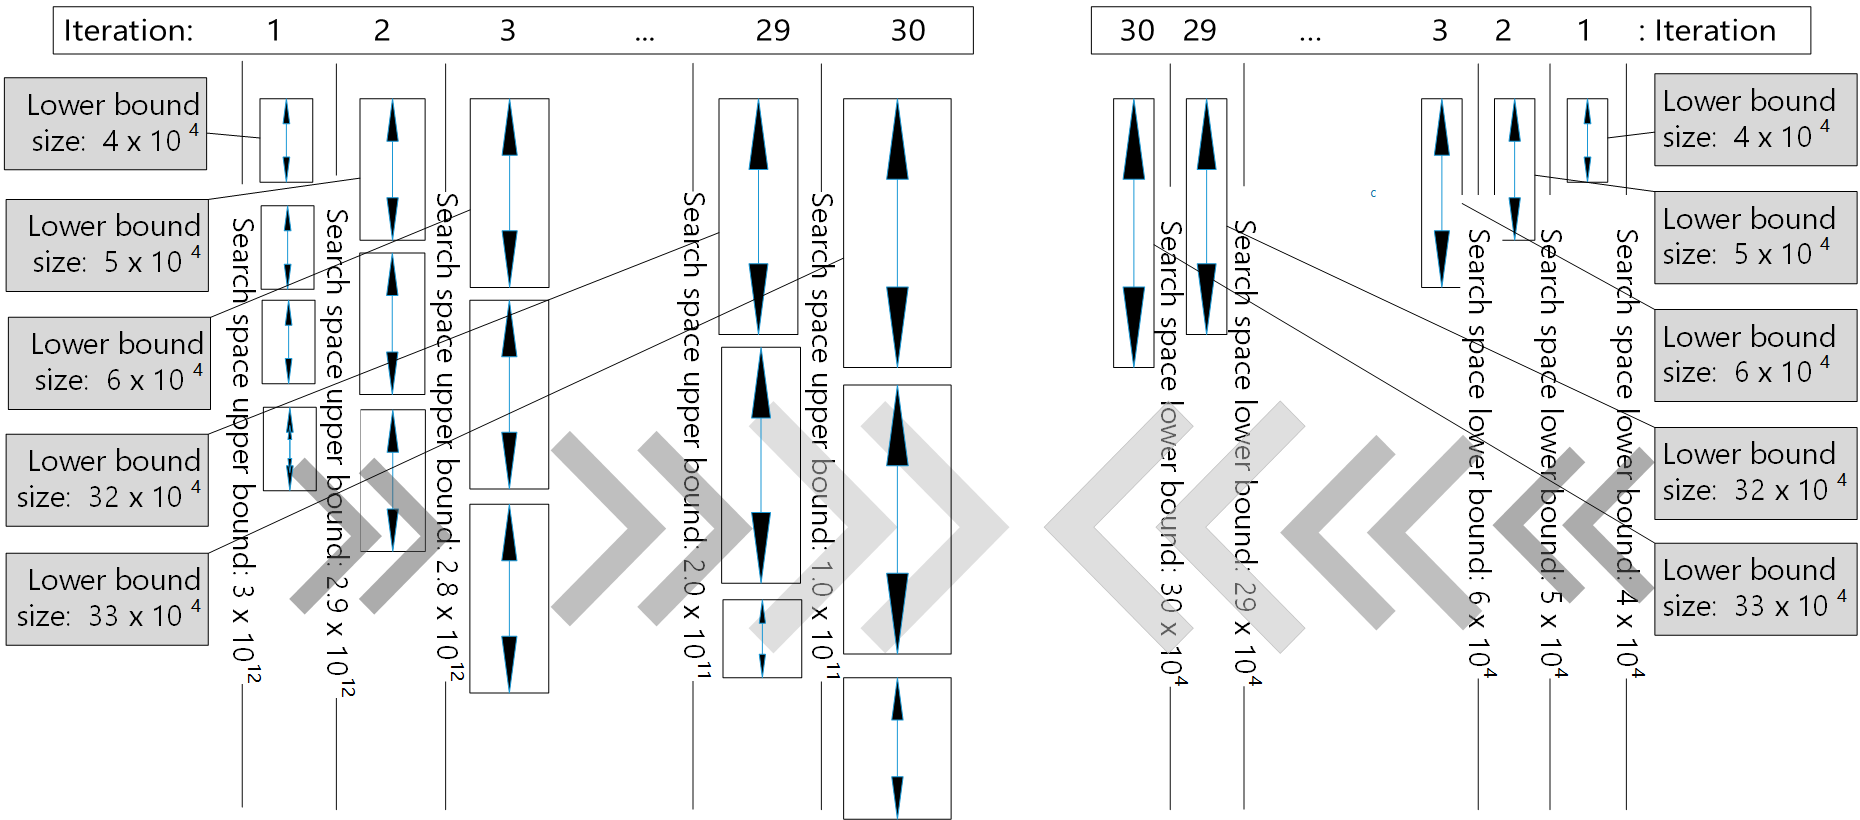
\includegraphics[scale=0.45]{figures/pincer.png}
 	\caption[]{Pincer Heuristic}
 	\label{fig:pincer}
 \end{figure}
%
%%%%%%%%%%%%%%%%%%%%%%%%%%%%%%%%%%%%%%%% ALGO 6 %%%%%%%%%%%%%%%%%%%%%%%%%%%%%%%%%%%%%%%%%%
%
\subsection{Backtracking Algorithm} \label{sec:backtracking}

In CSP it is common to find variables that have domain size 1, such variables are designated by singletons. Since both heuristics are based in constraint satisfaction programming, the rotations that we know in advance having variables with domain size 1, are handled first. In case of rotations with schedule maintenance, the algorithm treats them as a flight without turn round time and with the same origin and destination.  Thus, when the algorithm creates the aircraft list, the first aircraft have scheduled maintenance. The flights that are disrupted with delays are designated by fixed flights and they too cannot be moved. In this case the domain is a singleton consisting of value \{0\} and if this value is infeasible, because there are no available departure and/or arrival airport capacity, the algorithm backtracks by removing the rotation of an aircraft that can release the necessary airport capacity.

%%%%%%%%%%%%%%%%%%%%%%%%%%%%%%%%%%%%%%% ALGORITHM 6 %%%%%%%%%%%%%%%%%%%%%%%%%%%%%%%%%%%%%%%

Algorithm \ref{algo:backtracking} receives as inputs the singleton list, the airport capacity, the ARP current solution, the rotation and the index of the first infeasibility. The algorithm will return the ARP solution without the rotation that will allow the singleton to become feasible and the updated aircraft list. This algorithm will loop while the singleton list is not empty and will verify if the first singleton's infeasibility is on the departure and/or in the arrival airport capacity. Depending on the situation the algorithm computes the airport time slot for the departure/arrival and based on the origin/destination airport searches the  aircraft to cancel. The algorithm will then remove the aircraft from the solution list, and the respective rotation from the ARP solution. Finally, we will use algorithm \ref{algo:flightDomains} to determine there are any more infeasible singletons.
\begin{algorithm}[H]
	\DontPrintSemicolon
	\KwInput{$ singletonList, \mathcal{A}, aircraftSolList, solutionARP, \sigma_p, index $}
	\KwOutput{$solutionARP, aircraftSolList$}
	\While{$ singletonList \ne \{\}$}{
		
		\If{$singletonList(0) = 'dep'$}{
			$startInt \gets 60 * int(singleton^d(0)/60)$\\
			$endInt \gets startInt + 60$\\
			$origin \gets singleton^o(0)$\\
			$flight2Cancel \gets solutionARP[(origin, startInt, endInt)]$\\
			$airc2Cancel \gets updateMulti(flight2Cancel, \mathcal{A}, solutionARP])$\\
			$aircraftSolList \gets aircraftSolList - airc2Cancel$\\
			$solutionARP.pop(airc2Cancel)$\\
			$flightRanges, singletonList, totalCombos \gets domainFlights(\sigma_p(i) \forall i \in [index, |\sigma_p|], \mathcal{A}, index)$\\
		}
		\If{$singleton(0) = 'arr'$}{
			$startInt \gets 60 * int(singleton^a(0)/60)$\\
			$endInt \gets startInt + 60$\\
			$destination \gets singleton^f(0)$\\
			$flight2Cancel \gets solutionARP[(destination, startInt, endInt)]$\\
			$airc2Cancel \gets updateMulti(flight2Cancel, \mathcal{A}, solutionARP)$\\
			$aircraftSolList \gets aircraftSolList - airc2Cancel$\\
			$solutionARP.pop(airc2Cancel)$\\
			$flightRanges, singletonList, totalCombos \gets domainFlights(\sigma_p(i) \forall i \in [index, |\sigma_p|], \mathcal{A}, index)$\\
		}

	}
	return $solutionARP, aircraftSolList$
	\caption{Backtracking}
	\label{algo:backtracking}
\end{algorithm}

%%%%%%%%%%%%%%%%%%%%%%%%%%%%%%%%%% ALGO 7 %%%%%%%%%%%%%%%%%%%%%%%%%%%%%%%%%%%%%%%%%%
\subsection{Taxi Flights Algorithm} \label{sec:taxiFlights}
After finding a feasible solution for the part of the rotation that was initially infeasible the algorithm tries to reconnect both parts but on occasions it is possible to find discontinuities between them. Algorithm \ref{algo:taxiFlights}  receives as inputs the set of aircraft disruptions, the set of distances, the origin airport, the recovered rotation the maximum flight number and returns the updated recovered rotation and the maximum flight number. Algorithm \ref{algo:taxiFlights} will either create a taxi flight to connect the first part of the rotation and the recovered one, or cancel flights in the recovered rotation until the continuity infeasibility is removed. 

%%%%%%%%%%%%%%%%%%%%%%%%%%%%%%%%% ALGORITHM 7 %%%%%%%%%%%%%%%%%%%%%%%%%%%%%%%%%%%%%%

\begin{algorithm}[]
	\DontPrintSemicolon
	\KwInput{$ \mathcal{B},\Delta, originAirport, \sigma_p, \mathcal{A}, M $}
	\KwOutput{$\sigma_p, M$}
	$originSlots \gets \mathcal{A}[originAirport]$ if $capDep > noDep $\\
	\For{$\sigma_p(i)$ in $\sigma_p$}{
		\If{$\sigma^o_p(i) = originAirport$}{
			return $\sigma_p$, M	
		}
		$\delta_{of} \gets \Delta(originAirport, \sigma^{o}_p(i))$\\
		
		$originSlotsUpper \gets  originSlots$ if $endInt > \sigma^d_p(i) - \delta_{of} -t_{rp}$\\
		$originSlotsLower \gets originSlots - originSlotsUpper - [\mathcal{B}^s_p, \mathcal{B}^e_p]$\\
		\If{$originSlotsLower = \{\} $}{
			cancel($\sigma_p(i)$)\\
			continue}
		$destinationSlots \gets \mathcal{A}[\sigma^o_p]$ if $capArr > noArr $\\
		$destinationSlotsUpper \gets  destinationSlots$ if $endInt > \sigma^d_p(i) -t_{rp}$\\
		$destinationSlotsLower \gets destinationSlots - destinationSlotsUpper - [\mathcal{B}^s_p, \mathcal{B}^e_p]$\\
		\If{$destinationSlotsLower = \{\} $}{
			cancel($\sigma_p(i)$)\\
			continue}
		$destIntervals \gets \{\}$\\
		$i \gets -1$\\
		$offset \gets -1$\\
		\For{$x \in destinationSlotsLower$}{
			$destIntervals \gets destIntervals \cup [x^s, x^e]$
		}
		\For{$os(i)$ in $originSlotsLower$}{
			$obj \gets interval(os^s, os^e) + distInitRot$\\
			$i, offset \gets obj.findIntersection(destIntervals)$\\
			\If{$i \ne -1$}{	
				$taxiFlight^o \gets originAirport$\\
				$taxiFlight^d \gets os['startInt'] + offset$\\
				$taxiFlight^f = \sigma^o_p(i)$\\
				$taxiFlight^a = taxiFlight^d + \delta_{of}$\\
				$taxiFlight['flight'] = M$\\
				$M \gets M + 1$\\
				$\sigma_p \gets \sigma_p + taxiFlight$\\
				return $\sigma_p, M$\\}
		}
	}
	\caption{Taxi flights}
	\label{algo:taxiFlights}
\end{algorithm}

It starts in line 1  initializing the origin slots where there is available departure capacity. Afterwards the algorithm will loop through the flights of the recovered rotation  and if their origin is the same as origin airport it returns the updated recovered rotation and the maximum flight number (lines 2 to 4). In line 5 the algorithm computes the distance from the origin airport and the origin of the flight in the recovered rotation. In line 6 the algorithm extracts the upper slots from the origin slots by subtracting to the flight's departure time in the recovered rotation the distance and the turn round time. In line 7 the upper slots and the aircraft breakdown period are subtracted to the origin slots in order to retrieve the lower slots from where the aircraft can depart. If there are no available departure slots the algorithm cancels the flight in the recovered rotation and continues to the next flight (lines 8 to 10). If there are available departure slots at the origin, the algorithm tries to find destination slots with available airport arrival capacity. To achieve the latter the algorithm finds the destination slots with available capacity, the upper destination slots, and by subtracting the latter to the former and aircraft breakdown period determines the lower destination slots (lines 11 to 13). If there are no lower destination slots, the algorithm cancels the flight in the recovered rotation and continues to the next flight. Since $\mathcal{A}$ is a dictionary, it is necessary to extract the destination intervals and initialize the destination index $i$ and the time offset from which the flight departs and arrives in feasible airport slots (lines 17 to 21). The algorithm will then loop through the destination slots and in line 23 it will initialize the object $obj$ with the starting and end time of the origin lower slots plus the distance and, in line 24 determine the index of intersection in the destination slot and the offset. If the index $i$ is different from -1 the algorithm will the taxi flight and add it to the recovered rotation (lines 25 to 33).\\ 

\subsection{The CHARP} \label{sec:charp}

In figure \ref{fig:mainAlgo} we provide the complete flowchart of the CHARP. Step 1 of the algorithm consists in loading the data set, after which it starts looping through the aircraft list. In step 2 the algorithm selects an aircraft, and verifies if the rotation has been initialized, if it has not in step 4 and 5 it lists the infeasibilities and adds new flights. If the aircraft's rotation has been initialized in step 6 the algorithm checks if there are infeasibilities and if there are none, in step 10 it updates the ARP's solution with the aircraft's rotation, the airport capacity and the aircraft's solution list. If there are infeasibilities the algorithm will, in step 70, find the flight domains and compute the search space size, after which it will choose solution method (steps 710 and 720) and if necessary, the algorithm backtracks.
%%%%%%%%%%%%%%%%%%%%%%%%%%%%%%%%%%%%%%%%%%%%%%%%%%%%%%%%%%%%%%%%%%%%%%
If the size of the search space is lower than the lower bound the algorithm uses the lower heuristic algorithm (step 723), if the search space size is bigger than the upper bound it will use the upper heuristic algorithm (step 713). If neither of the previous apply the algorithm verifies if the loop has finished and if it has not it will move to the next aircraft. After recovering the infeasible part of the rotation, the algorithm checks in step 8, if there is a continuity infeasibility when it tries to reconnect both parts. If there is, in step 9 the taxi flights algorithm reconnects both parts and afterwards adds the recovered rotation to the solution, updates the airport capacity and updates the aircraft solution list (step 10). In step 11  the algorithm checks if the loop has finished aircraft list and if it has it checks if there are any aircraft left to recover (step 12). If there are the algorithm updates the lower and the upper bound and iterates. If there are no more aircraft the algorithm ends.

 \begin{figure}[h!]
	\centering
	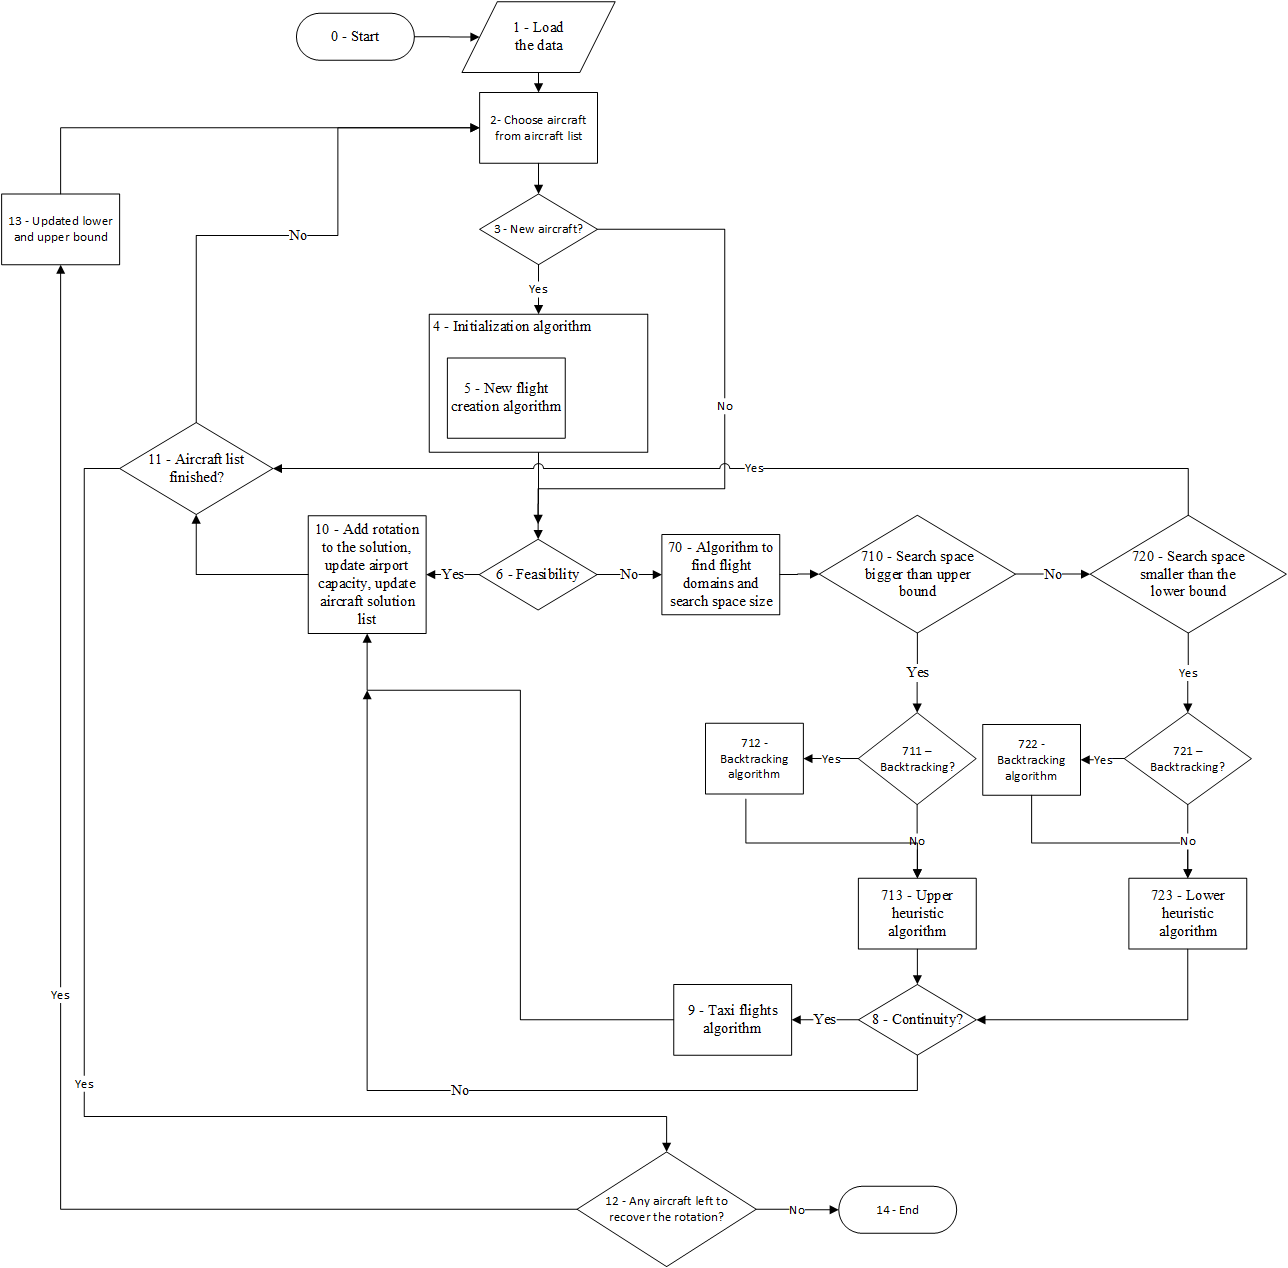
\includegraphics[scale=0.65]{figures/mainAlgo.png}
	\caption[]{Constructive Heuristic}
	\label{fig:mainAlgo}
\end{figure}

%\end{document}


\section{Computational Results}\label{sec:compResults}

\hl{In this section, we aim at studying the cost and the computing time of the CHARP for the overall 32 data instances of the ROADEF 2009 Challenge.  To obtain the computing time, we run all 32 instances simultaneously and we retrieve the computing time of the last one being solved. As for the cost we use the cost checker application provided by the ROADEF 2009 Challenge. The remainder of this section consists of, Section} \ref{sec:impact} \hl{ where we will demonstrate the impact of adding new flights and taxi flights. Since the heuristic performs a pincer movement in Section} \ref{sec:pincerSpeed} \hl{we will determine which is the best speed by changing the decremental and incremental steps.}\\
 
%All the models and algorithms were written in Python language. The scripts were implemented on a computer with 4-core processors running at 2.3  GHz and 16 GB memory.\\


\subsection{The Impact of New Flights and Taxi Flights}\label{sec:impact}

  
\subsection{The Impact of the Pincer Speed}\label{sec:pincerSpeed}

 







\section{Conclusions}\label{sec:conclusions}

ARP is a practical problem that needs to be solved during operations, therefore, the efficiency of the method in terms of computational time is a very important characteristic.
The CHARP loads the respective data, introduces the disruptions and if necessary allocates times slots for new flights. We then select a sub-rotation starting in infeasible flight and proceed to recover it. The recovery procedure is done using an upper or a lower heuristic depending on the size of the search space. The recovery procedure will afterwards try to reconnect the first part of the rotation with the recovered one and for this purpose, if necessary, create taxi flights. In the impossibility of the latter the algorithm will cancel the flights in the recovered rotation until the continuity constraint be satisfied.The data instance vary in size comprising a number of flights from 608 to  2178, aircraft from 85 to 618 and airport from 35 to 168.
 Most of the works in the literature reach computational times of less than thirty minutes, however it is important that this limit is possible for large instances, that is, those with more than 400 flights. In this work we achieve this goal with a novel heuristic based in CSP. One factor that facilitates these objectives is the greater availability of high-performance computing infrastructure. Our experiments were conducted in an Intel Xeon Gold CPU @ 2.3GHz box which allowed to run simultaneously 320 scenarios for every CHARP speed.
We were able to find solutions, in less than 30 minutes, the best having a speed of 0.5 for a time window of 900 minutes. 



% Appendix here
% Options are (1) APPENDIX (with or without general title) or
%             (2) APPENDICES (if it has more than one unrelated sections)
% Outcomment the appropriate case if necessary
%
% \begin{APPENDIX}{<Title of the Appendix>}
% \end{APPENDIX}
%
%   or
%
% \begin{APPENDICES}
% \section{<Title of Section A>}
% \section{<Title of Section B>}
% etc
% \end{APPENDICES}


% Acknowledgments here
%\ACKNOWLEDGMENT{The authors gratefully acknowledge the existence of
%the Journal of Irreproducible Results and the support of the Society
%for the Preservation of Inane Research.}


% References here (outcomment the appropriate case)

% CASE 1: BiBTeX used to constantly update the references
%   (while the paper is being written).
\bibliographystyle{informs2014} % outcomment this and next line in Case 1
\bibliography{myLibrary} % if more than one, comma separated

% CASE 2: BiBTeX used to generate mypaper.bbl (to be further fine tuned)
%\input{mypaper.bbl} % outcomment this line in Case 2

%If you don't use BiBTex, you can manually itemize references as shown below.


%\bibliographystyle{nonumber}
%\bibliography{myLibrary}

%%%%%%%%%%%%%%%%%
\end{document}
%%%%%%%%%%%%%%%%%

